\documentclass[tikz,border=6pt]{standalone}

\usepackage[T1]{fontenc}
\usepackage{lmodern}
\usepackage{xcolor}
\usetikzlibrary{shapes,arrows,positioning,calc}

\begin{document}
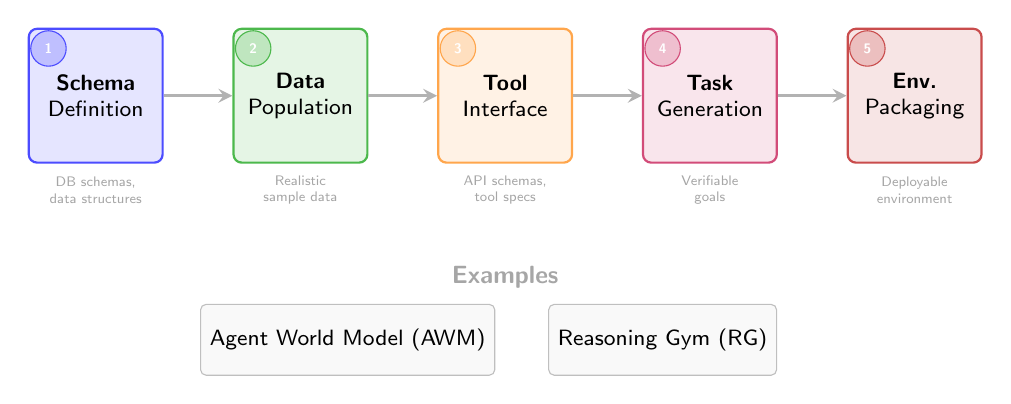
\begin{tikzpicture}[
    step/.style={rectangle, draw=#1!70, fill=#1!10, minimum width=1.7cm, minimum height=1.7cm, align=center, font=\footnotesize\sffamily, thick, rounded corners=3pt},
    num/.style={circle, draw=#1!70, fill=#1!25, minimum size=0.45cm, font=\tiny\sffamily\bfseries, text=white, inner sep=0pt},
    arr/.style={->, >=stealth, thick, color=gray!60, line width=1.2pt},
    exbox/.style={rectangle, draw=gray!50, fill=gray!5, minimum width=2.5cm, minimum height=0.9cm, align=center, font=\footnotesize\sffamily, rounded corners=2pt}
]
% Steps
\node[step=blue] (s1) at (0,0) {\textbf{Schema}\\Definition};
\node[step=green!60!black] (s2) at (2.6,0) {\textbf{Data}\\Population};
\node[step=orange] (s3) at (5.2,0) {\textbf{Tool}\\Interface};
\node[step=purple] (s4) at (7.8,0) {\textbf{Task}\\Generation};
\node[step=red!70!black] (s5) at (10.4,0) {\textbf{Env.}\\Packaging};

% Step numbers
\node[num=blue] at (-0.6,0.6) {1};
\node[num=green!60!black] at (2.0,0.6) {2};
\node[num=orange] at (4.6,0.6) {3};
\node[num=purple] at (7.2,0.6) {4};
\node[num=red!70!black] at (9.8,0.6) {5};

% Arrows
\draw[arr] (s1) -- (s2);
\draw[arr] (s2) -- (s3);
\draw[arr] (s3) -- (s4);
\draw[arr] (s4) -- (s5);

% Sub-labels
\node[font=\tiny\sffamily, text=gray!70, align=center] at (0,-1.2) {DB schemas,\\data structures};
\node[font=\tiny\sffamily, text=gray!70, align=center] at (2.6,-1.2) {Realistic\\sample data};
\node[font=\tiny\sffamily, text=gray!70, align=center] at (5.2,-1.2) {API schemas,\\tool specs};
\node[font=\tiny\sffamily, text=gray!70, align=center] at (7.8,-1.2) {Verifiable\\goals};
\node[font=\tiny\sffamily, text=gray!70, align=center] at (10.4,-1.2) {Deployable\\environment};

% Examples
\node[font=\small\sffamily\bfseries, text=gray!70] at (5.2,-2.3) {Examples};
\node[exbox] at (3.2,-3.1) {Agent World Model (AWM)};
\node[exbox] at (7.2,-3.1) {Reasoning Gym (RG)};
\end{tikzpicture}
\end{document}